
\section{Vacuum Photo-triodes}
\label{sec:eq_vpt}

The electromagic calorimeter (Ecal) is composed of scintillators and scintillator detectors.  The scintilators are transparent PbWO$_4$ crystals.  These crystals are relatively weak scintillators, producing only \~{}50\,photons per MeV. [\href{papers/1344324}{K.W.\ Bell,~et~al.}]  As such, to reach the energy resolutions needed by CMS the photodetectors must have a built-in gain mechanism with low noise production.  In the barrel of CMS, Avalance Photo-Diodes (APDs) are used.  However, in endcap, where radiation levels much higher, Vacuum Photo-Triodes (VPTs) are used.

\begin{figure}[htbp]
  \centering
  \pgfimage[interpolate=true,height=3in]{figures/IMG_4261}
  \caption{Photograph of Vacuum Photo-Triode}
  \label{fig:eq_vpt:vpt}
\end{figure}

A Vacuum Photo-Triode (VPT) is a specific electronic light sensor with a built-in photo-electron multiplier effect.  Like a photodiode, it exploits the photoelectric effect to liberate electrons with incoming photons.  As photons strike the photocathode, electrons are ejected.  (The photocathode has effectively infinite current to replenish its electrons.)  In addition to the energy from the incident photon, the electrons are imparted with an additional 1400\,eV of potential energy from the high voltage applied to the anode and dynode.  

\begin{figure}[htbp]
  \centering
    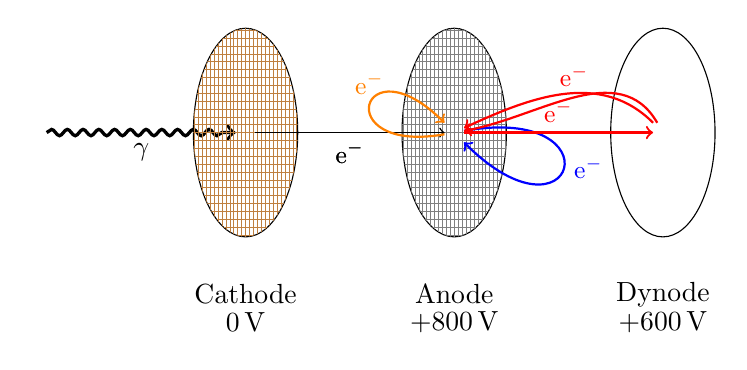
\begin{tikzpicture}

    \node (light) at (-26.5mm*2,0) {};

    \node (cathode) at (-26.5mm,0) {};
    \path (cathode) ++(down:27mm/2 + 2em) node (cathode label) {Cathode};
    \path (cathode label) ++(down:1em) node (cathode voltage) {0\,V};

    \node (anode) at (0,0) {};
    \path (anode) ++(down:27mm/2 + 2em) node (anode label) {Anode};
    \path (anode label) ++(down:1em) node (anode voltage) {$+$800\,V};

    \node (dynode) at (26.5mm,0) {};
    \path (dynode) ++(down:27mm/2 + 2em) node (dynode label) {Dynode};
    \path (dynode label) ++(down:1em) node (dynode voltage) {$+$600\,V};

    % Incoming Light
    \path[->] (light) edge[very thick,decorate,decoration={snake,amplitude=.4mm,segment length=2mm,post length=1mm}] node[below,sloped] {$\gamma$} (cathode);
  
    % Cathode Mesh
    \begin{scope}[xscale=.5]
      \draw[clip] (cathode) circle (26.5mm/2);
      \draw[step=1mm,help lines,xshift=-26.5mm*2,brown] (-27mm/2,-27mm/2) grid (27mm/2,27mm/2);
    \end{scope}

    % Anode Mesh
    \begin{scope}[xscale=.5]
      \draw[clip] (anode) circle (26.5mm/2);
      \draw[step=1mm,help lines] (-27mm/2,-27mm/2) grid (27mm/2,27mm/2);
    \end{scope}

    % Dynode Plate
    \begin{scope}[xscale=.5]
      \draw[thin] (dynode) circle (26.5mm/2);
    \end{scope}

    \path[->] (cathode) edge[thin] node[below] {\small e$^-$} (anode);
    \path[->] (cathode) edge[thin] node[below] {\small e$^-$} (anode);

    \begin{scope}[every loop/.style={min distance=20mm}]
      % \path[->,thick] (anode) edge [out=-10,in=45,loop] node[right] {\small e$^-$} ();
      \path[->,thick,blue] (anode) edge [out=10,in=-45,loop] node[right] {\small e$^-$} ();
      \path[->,thick,orange] (anode) edge [distance=15mm,out=190,in=-225,loop] node[above] {\small e$^-$} ();
      \path[->,thick,red] (anode) edge [] node[above] {\small e$^-$} (dynode);
      \path[->,thick,red] (dynode) edge [out=120,in=10] node[above] {\small e$^-$} (anode);
      \path[->,thick,red] (dynode) edge [out=135,in=25] node[above] {\small } (anode);
    \end{scope}
    
  \end{tikzpicture}

  \caption{VPT Electron Action}
  \label{fig:eq_vpt:electron_action}
\end{figure}

The emitted photoelectron falls towards the anode and may miss the anode mesh and collide with the dynode, causing secondary electron emissions which will fall back towards the anode.  If the initial photoelectron hits the anode mesh, it may also cause secondary emissions which will impact the dynode and cause tertiary emissions to fall back to the dynode.  The electrons continue falling up and down the potential energy well causing secondary emissions until their kinetic energy at the anode is less than the work function, and so get absorbed without secondary emissions.  This results in a rapid rise in output (anode) current followed by a slower fall off.  This process is extremely fast, returning to zero current from a pulse of 420\,nm light in around 200\,ns.

The 200\,ns response time of VPTs makes them acceptable for use in CMS, which operates at 40\,MHz ($T=25\,\mathrm{ns}$).  The chance of beam products interacting with the same barrel crystal before complete recovery is small, and the occasional overlapping event can be detected and accounted for.


\begin{figure}[htbp]
  \centering
    \begin{tikzpicture}[yscale=-1]
    \draw[->] (0,26.5mm) -- (0,-5mm) node[left] {$U(x)$};
    \draw[->] (0,26.5mm/2) -- (26.5mm*2,26.5mm/2) node[right] {$x$};
    % \draw[very thin, color=gray, step=26.5mm/7]
    %   (-1mm,-1mm) grid (26.5mm*2-1mm,26.5mm+1mm);

    \node[anchor=west,rotate=-60] at (0,26.5mm) {Cathode};
    \node[anchor=west,rotate=-60] at (26.5mm*1,26.5mm) {Anode};
    \node[anchor=west,rotate=-60] at (26.5mm*2,26.5mm) {Dynode};

    \draw[color=red]
       (0,0) -- (26.5mm*1,26.5mm) -- (26.5mm*2,26.5mm*4/7);
  \end{tikzpicture}

  \caption{VPT Electron Potential Well (qualitative)}
  \label{fig:eq_vpt:vpt_potential}
\end{figure}

\begin{figure}[htbp]
  \centering
  {
    \tiny Taken from \href{papers/VPT_Phys393}{Christine Drown's PHY 393 Spring 2008 Paper}\\
  }
  \pgfimage[interpolate=true,height=3in]{figures/christine_drown_vpt_pulse}
  \caption{VPT Pulse Shape}
  \label{fig:eq_vpt:vpt_pulse}
\end{figure}

When we test a VPT at HEP, we send a pulse of light from a single source (an LED) down at least two different fibers.  One fiber illuminates the photocathode of the VPT, while the other illuminates a standardized PIN diode.  We use the PIN diode's output as a reference for the light input to the VPT.  We can then calculate the gain, or the amount of charge amplification the VPT provides.

VPTs have a number of interesting characteristics that need to be studied.  One of the reasons VPTs were chosen is that they continue to function in strong non-axial magnetic fields, due to their single-stage photomultiplier design.  However, they still exhibit varibility in their response within non-axial magnetic fields.  The field in CMS is not entirely uniform between the beam axis and the outer edges of the endcap.  Therefore, the relative gain of each VPT is affected by the direction of the magnetic field, which varies continuously depending on how far from the beam axis the VPT is placed.

\begin{figure}[htbp]
  \centering
  \pgfimage[interpolate=true,height=3in]{figures/13May_VPT1_resp}
  \caption{VPT Angle Repsponse Example}
  \label{fig:eq_vpt:vpt_angle_response}
\end{figure}

VPTs also demonstrate a burn-in effect which can sometimes be quite pronounced.  The amplification VPTs produce degrades over time, so that the same pulsed photocurrent will result in less output days later.  The effect is not permanent, however.  The self-correcting behavior of VPTs was being studied at UVA in 2009 when an electrical failure of the old NIM crate damaged several instruments and interrupted the experiment.

\begin{figure}[htbp]
  \centering
  \pgfimage[interpolate=true,height=3in]{figures/Anode_PIN_Corrected_linear}
  \caption{VPT Long Term Effect}
  \label{fig:eq_vpt:vpt_long_term}
\end{figure}

\subsection{Further Reading}
\label{sec:eq_vpt:reading}

\begin{itemize}
\item D.C. Imrie. \href{papers/VPT Burn-in}{Long-Term Behaviour Of Three Prototype Vacuum Phototriodes Operated With High Photocurrents}. January 2000.
\item M.N. Achasov, et~al. \href{papers/0102083v1-1}{Compact Vacuum Phototriodes for operation in strong magnetic field}.  26 February 2001.
\item K.W. Bell, et~al. \href{papers/1344324}{Vacuum Phototriodes for the CMS Electromagnetic Calorimeter Endcap}.  October 2004.
\item P.Adzic, et~al. \href{papers/jinst8_10_p10007}{Intercalibration of the barrel electromagnetic calorimeter of the CMS experiment at start-up}. October 2008.
\end{itemize}

\subsubsection{At UVA}
\begin{itemize}
\item C. Drown.  \href{papers/VPT_Phys393}{Properties of Vacuum Photo-Triodes in a 4\,T Magnetic Field}.  Spring 2008.
\item D.G. Phillips II, et~al. \href{papers/newvptpaper}{A Measurement of the Temperature Stability of Vacuum Phototriodes for the CMS ECAL}.
\item J.C. Jones. \href{papers/Long Term VPT Response of Vacuum Photo-Triodes}{Long Term VPT Response of Vacuum Photo-Triodes}. Fall 2008.
\end{itemize}

%%% Local Variables: 
%%% mode: latex
%%% TeX-master: "Manual"
%%% End: 
